\documentclass[11pt,aspectratio=43]{beamer}

% Packages
\usepackage[utf8]{inputenc}
\usepackage[T1]{fontenc}
\usepackage{amsmath,booktabs,array,tabularx}
\usepackage{graphicx,tikz,xcolor}
\usepackage{listings}

% Theme
\usetheme{default}
\usecolortheme{default}
\setbeamertemplate{navigation symbols}{}
\setbeamertemplate{footline}[frame number]
\setbeamertemplate{caption}[numbered]
\setbeamerfont{frametitle}{series=\bfseries}

% Colors
\definecolor{aggiemaroon}{HTML}{500000}
\definecolor{codebg}{HTML}{F7F7F7}
\definecolor{codecomment}{RGB}{115,115,115}
\definecolor{codeblue}{RGB}{0,0,140}
\definecolor{codegreen}{RGB}{0,107,0}
\definecolor{coderule}{RGB}{190,190,190}

\setbeamercolor{structure}{fg=aggiemaroon}
\setbeamercolor{title}{fg=aggiemaroon}
\setbeamercolor{frametitle}{fg=aggiemaroon}

% Python code
\lstdefinestyle{python}{
  language=Python,
  backgroundcolor=\color{codebg},
  basicstyle=\ttfamily\scriptsize,
  keywordstyle=\color{codeblue}\bfseries,
  commentstyle=\color{codecomment}\itshape,
  stringstyle=\color{codegreen},
  showstringspaces=false,
  breaklines=true,
  frame=single,
  rulecolor=\color{coderule},
  framesep=3pt,
  xleftmargin=2pt,
  xrightmargin=2pt,
  tabsize=2,
  columns=fullflexible
}
\lstset{style=python}

% Tables
\newcolumntype{Y}{>{\raggedright\arraybackslash}X}

% Metadata
\title{Python Pandas}
\subtitle{Data Transformation: Grouping, Pivoting, Strings, Pipelines}
\author{}
\date{
  \textcolor{aggiemaroon}{
    DAEN 300\\
    \textbf{Alexander Abuabara}\\
    Fall 2026
  }
}
\titlegraphic{%
  \IfFileExists{TAMU_logo.png}
    {
\includegraphics[height=1.2cm]{TAMU_logo.png}}{}
}

\begin{document}

% ---------------------------------------------------
\begin{frame}
  \titlepage
\end{frame}

% ---------------------------------------------------
\begin{frame}{Outline}
  \tableofcontents
\end{frame}

% =====================================================
\section{Setup and Inspection}

\begin{frame}[fragile]{"Dataset" for Examples}
  \begin{lstlisting}
import pandas as pd
# load pandas with the standard alias pd

import numpy as np
# load NumPy

df = pd.DataFrame({
    'region': ['East','East','West','West','East'],
    'category': ['A','B','A','B','A'],
    'store': ['S1','S1','S2','S2','S3'],
    'price': [10, 20, 30, 40, 50],
    'qty': [1, 2, 3, 4, 5],
    'name': [' ada lovelace ', 'Grace Hopper', None,
             'Alan Turing', 'Katherine Johnson']
})
  \end{lstlisting}
\end{frame}

\begin{frame}[fragile]{Pandas}
  \begin{itemize}
    \item Work with labeled tables instead of raw arrays.
    \item Clean, reshape, join, aggregate, and analyze data quickly.
    \item Use vectorized operations whenever possible for speed and clarity.
  \end{itemize}
  \vspace{0.4em}
  \begin{lstlisting}
s = df['price']
# a Series; one labeled column from the table

small = df[['region', 'price']]
# a DataFrame with two selected columns
  \end{lstlisting}
\end{frame}

\begin{frame}[fragile]{Inspection}
  \begin{lstlisting}
df.head()
# returns the first 5 rows; useful first look

df.info()
# shows columns, dtypes, memory, and non-null counts

df.describe()
# price mean = 30.0, qty mean = 3.0 in the toy data

df.shape
# (5, 6), meaning 5 rows and 6 columns

df.sample(2, random_state=1)
# two random rows; avoids only seeing the top of the file

df.dtypes
# price and qty are int64; name is object/string-like
  \end{lstlisting}
\end{frame}

% =====================================================
\section{Selecting and Filtering}

\begin{frame}[fragile]{Selection: \texttt{loc} vs \texttt{iloc}}
  \begin{lstlisting}
df.loc[0, 'price']
# 10; label-based row/column lookup

df.iloc[0, 3]
# 10; position-based lookup, row 0 and column 3

df.loc[df['price'] > 25, ['region', 'price']]
# rows with prices 30, 40, and 50

mask = (df['price'] > 25) & (df['category'] == 'A')
# True for the West-A row and East-A row with price 50

df[mask]
# keeps only rows where the mask is True
  \end{lstlisting}
  Use \texttt{\&} and \texttt{|}, not \texttt{AND} and \texttt{OR}; wrap each condition in parentheses.
\end{frame}

\begin{frame}[fragile]{Readable Filters with \texttt{query}}
  \begin{lstlisting}
df.query('price > 25 and category == "A"')
# returns rows with price 30 and 50 in category A

threshold = 25
# create a Python variable for the cutoff

df.query('price > @threshold')
# @threshold injects the Python variable into the query
  \end{lstlisting}
  \begin{itemize}
    \item Good for long filters and method chains.
    \item Column names with spaces require backticks, for example \texttt{`unit price`}.
  \end{itemize}
\end{frame}

% =====================================================
\section{GroupBy}

\begin{frame}[fragile]{GroupBy Basics}
  \begin{lstlisting}
df.groupby('category')['price'].mean()
# A -> 30.0, B -> 30.0

df.groupby('category').agg(
    avg_price=('price', 'mean'),
    orders=('price', 'size'),
    max_price=('price', 'max')
)
# clean columns named avg_price, orders, max_price
  \end{lstlisting}
  Named aggregation avoids messy MultiIndex column names.
\end{frame}

\begin{frame}[fragile]{GroupBy: Multiple Columns and Functions}
  \begin{lstlisting}
df.groupby(['region', 'category'])['price'].sum()
# East/A -> 60, East/B -> 20, West/A -> 30, West/B -> 40

df.groupby(['region', 'category']).agg(
    total_sales=('price', 'sum'),
    total_qty=('qty', 'sum')
)
# one row per region-category combination

df.groupby('category')['price'].agg(['mean', 'min', 'max'])
# A has min 10 and max 50; B has min 20 and max 40
  \end{lstlisting}
\end{frame}

\begin{frame}[fragile]{Lambda}
  \begin{lstlisting}
lambda x: x * 2
# an anonymous function; input x, output x * 2

(lambda x: x * 2)(5)
# 10

def double(x):
    return x * 2
# same logic as lambda x: x * 2, but with a name
  \end{lstlisting}
  \begin{itemize}
    \item Syntax: \texttt{lambda argument: expression}.
    \item A lambda has exactly one expression, not a full block of statements.
    \item In pandas, the argument is often a row, Series, group, or DataFrame.
  \end{itemize}
\end{frame}

\begin{frame}[fragile]{Lambda in GroupBy}
  \begin{lstlisting}
df.groupby('category')['price'].apply(lambda s: s.max() - s.min())
# A -> 40, B -> 20; range of prices by category

df.groupby('category').filter(lambda g: len(g) >= 2)
# keeps A and B because each category has at least 2 rows

df.groupby('category')['price'].transform(lambda s: s - s.mean())
# subtracts each category mean from each row's price
  \end{lstlisting}
  \textbf{Interpretation:} \texttt{s} is one category's price Series; \texttt{g} is one category's DataFrame.
\end{frame}

\begin{frame}[fragile]{GroupBy Tricks: \texttt{transform} and \texttt{filter}}
  \begin{lstlisting}
df['cat_total'] = df.groupby('category')['price'].transform('sum')
# category A rows receive 90; category B rows receive 60

df['pct_of_cat'] = df['price'] / df['cat_total']
# first row is 10 / 90 = 0.111...

df.groupby('category').filter(lambda g: g['price'].mean() >= 30)
# keeps categories whose average price is at least 30
  \end{lstlisting}
  \texttt{transform} returns one value per original row, so it is ideal for adding group-level columns.
\end{frame}

\begin{frame}[fragile]{Top Values per Group}
  \begin{lstlisting}
df['category'].value_counts(normalize=True)
# A -> 0.60, B -> 0.40

df.groupby('category')['price'].apply(lambda s: s.nlargest(2))
# top two prices inside each category

df.sort_values('price').groupby('category').tail(1)
# max-price row for A is 50; max-price row for B is 40
  \end{lstlisting}
\end{frame}

% =====================================================
\section{Pivoting and Reshaping}

\begin{frame}[fragile]{Pivot Tables}
  \begin{lstlisting}
pd.pivot_table(
    df,
    index='region',
    columns='category',
    values='price',
    aggfunc='mean'
)
# rows are East/West; columns are A/B; cells are mean price
  \end{lstlisting}
  \begin{itemize}
    \item \texttt{index}: rows in the result.
    \item \texttt{columns}: values spread across columns.
    \item \texttt{aggfunc}: how duplicate cells are summarized.
  \end{itemize}
\end{frame}

\begin{frame}[fragile]{Pivot Tables: Practical Options}
  \begin{lstlisting}
pd.pivot_table(
    df,
    index=['region', 'store'],
    columns='category',
    values=['price', 'qty'],
    aggfunc={'price': 'mean', 'qty': 'sum'},
    margins=True,
    fill_value=0
)
# adds All totals and replaces missing cells with 0
  \end{lstlisting}
  \small
  \texttt{margins=True} gives row and column totals without a separate calc.
\end{frame}

\begin{frame}[fragile]{\texttt{pivot}, \texttt{pivot\_table}, \texttt{crosstab}}
  \begin{lstlisting}
df.pivot(index='store', columns='category', values='price')
# reshapes only if each store-category pair is unique

pd.crosstab(df['category'], df['region'])
# frequency table: category by region

pd.crosstab(df['category'], df['region'], normalize='index')
# row percentages that sum to 1.0 within each category
  \end{lstlisting}
\end{frame}

\begin{frame}[fragile]{Reshaping: \texttt{melt}, \texttt{stack}, \texttt{unstack}}
  \begin{lstlisting}
wide = pd.DataFrame({'id': [1, 2], 'jan': [10, 20], 'feb': [30, 40]})
# sales are stored across month columns

pd.melt(wide, id_vars='id', value_vars=['jan', 'feb'],
        var_name='month', value_name='sales')
# converts jan/feb columns into month and sales rows

df.set_index(['region', 'category'])['price'].unstack('category')
# category values become columns A and B
  \end{lstlisting}
\end{frame}

% =====================================================
\section{String Operations}

\begin{frame}[fragile]{\texttt{.str}}
  \begin{lstlisting}
df['name'].str.lower()
# 'Grace Hopper' becomes 'grace hopper'

df['name'].str.strip()
# ' ada lovelace ' becomes 'ada lovelace'

df['name'].str.contains('hopper', case=False, na=False)
# True for Grace Hopper; False for missing names

df['name'].str.replace(r'\s+', ' ', regex=True)
# collapses repeated spaces into one space

df['name'].str.len()
# counts characters, including leading/trailing spaces
  \end{lstlisting}
\end{frame}

\begin{frame}[fragile]{String Tricks: Split and Extract}
  \begin{lstlisting}
clean_name = df['name'].str.strip()
# remove extra spaces before splitting

df[['first', 'last']] = clean_name.str.split(' ', n=1, expand=True)
# 'Ada Lovelace' -> first='Ada', last='Lovelace'

df['first_initial'] = df['first'].str.extract(r'^(\w)')
# Ada -> A, Grace -> G

df['words'] = clean_name.str.count(r'\w+')
# 'Katherine Johnson' has 2 words
  \end{lstlisting}
\end{frame}

\begin{frame}[fragile]{String Tricks: Join, Pad, Case}
  \begin{lstlisting}
df['full'] = df['first'].str.cat(df['last'], sep=' ')
# first='Grace', last='Hopper' -> 'Grace Hopper'

df['code'] = df.index.astype(str).str.zfill(3)
# index 7 would become '007'

df['title'] = df['name'].str.strip().str.title()
# ' ada lovelace ' -> 'Ada Lovelace'

df['slug'] = df['title'].str.lower().str.replace(r'\W+', '-', regex=True)
# 'Grace Hopper' -> 'grace-hopper'
  \end{lstlisting}
\end{frame}

\begin{frame}[fragile]{Categorical Dtype for Repeated Strings}
  \begin{lstlisting}
df['category'] = df['category'].astype('category')
# stores repeated A/B values more compactly than object strings

df['size'] = pd.Categorical(
    ['S','M','L','M','S'],
    categories=['S','M','L','XL'],
    ordered=True
)
# sorting respects S < M < L < XL
  \end{lstlisting}
  \begin{itemize}
    \item Useful for low-cardinality text columns.
    \item Can improve memory use and some grouping/sorting operations.
  \end{itemize}
\end{frame}

{\setbeamercolor{background canvas}{bg=gray!20}

  \begin{frame}[fragile]{Comparing Object Sizes}
    \footnotesize
    \begin{lstlisting}
import sys
import numpy as np

vector_a = [1, 2, 3, 4, 5]
array_b  = np.array([1, 2, 3, 4, 5])

sys.getsizeof(vector_a)  # list object
sys.getsizeof(array_b)   # NumPy array object
array_b.nbytes           # raw array data
    \end{lstlisting}

    \begin{itemize}
      \small
      \item \texttt{sys.getsizeof()} measures the Python object itself.
      \item \texttt{vector\_a} is a list of references to Python objects.
      \item \texttt{array\_b} stores values in a compact contiguous data block.
      \item \texttt{array\_b.nbytes} reports only the raw numeric data size.
    \end{itemize}
  \end{frame}


  \begin{frame}[fragile]{Object Size vs. Data Size}
    \footnotesize
    Object size includes the container/metadata overhead,\\
    while data size measures only the memory occupied by the stored values.

    \begin{lstlisting}
array_b = np.array([1, 2, 3, 4, 5])

array_b.size      # number of elements
array_b.itemsize  # bytes per element
array_b.nbytes    # size * itemsize
    \end{lstlisting}

    \[
    \texttt{array\_b.nbytes}
    =
    \texttt{array\_b.size}
    \times
    \texttt{array\_b.itemsize}
    \]

    \begin{itemize}
      \small
      \item \texttt{sys.getsizeof(array\_b)} includes array-object overhead.
      \item \texttt{array\_b.nbytes} includes only the data buffer.
      \item Metadata such as shape, dtype, and strides is not included in \texttt{nbytes}.
    \end{itemize}
  \end{frame}

  \begin{frame}[fragile]{Why Lists Do Not Have \texttt{nbytes}}
    \footnotesize
    \begin{lstlisting}
vector_a = [1, 2, 3, 4, 5]

sys.getsizeof(vector_a)  # list container + references
vector_a.nbytes          # AttributeError
    \end{lstlisting}

    \begin{center}
      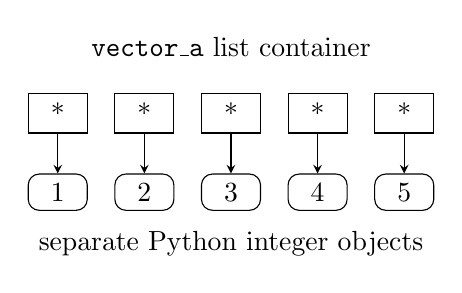
\begin{tikzpicture}[
        ref/.style={draw, minimum width=0.75cm, minimum height=0.45cm},
        obj/.style={draw, rounded corners, minimum width=0.75cm, minimum height=0.45cm},
        >=stealth
        ]
        \node at (2.2,0.85) {\texttt{vector\_a} list container};

        \foreach \x/\val in {0/1,1/2,2/3,3/4,4/5} {
          \node[ref] (r\x) at (\x*1.1,0) {*};
          \node[obj] (o\x) at (\x*1.1,-1.0) {\val};
          \draw[->] (r\x.south) -- (o\x.north);
        }

        \node at (2.2,-1.65) {separate Python integer objects};
      \end{tikzpicture}
    \end{center}
    \begin{itemize}
      \small
      \item \texttt{nbytes} is specific to NumPy arrays.
      \item Lists store references, not compact raw values.
      \item \texttt{sys.getsizeof(vector\_a)} is not recursive
      \tiny{... it measures only the memory used directly by the list container, not the memory used by the objects referenced inside the list}.
    \end{itemize}
  \end{frame}
}

% =====================================================
\section{Chaining and Performance}

\begin{frame}[fragile]{Method Chaining with \texttt{assign}}
  \begin{lstlisting}
result = (
    df
    .query('price > 0')
    # keep valid positive prices
    .assign(
        revenue=lambda d: d['price'] * d['qty'],
        # lambda d sees the current DataFrame in the chain
        price_band=lambda d: np.where(d['price'] >= 30, 'high', 'low')
        # price 10/20 -> low; price 30/40/50 -> high
    )
    .groupby('price_band')['revenue'].sum()
    # total revenue by price band
    .sort_values(ascending=False)
    # largest revenue band first
)
  \end{lstlisting}
\end{frame}

\begin{frame}[fragile]{Performance: Vectorize, Do Not Loop}
  \begin{lstlisting}
df['total_slow'] = df.apply(lambda r: r['price'] * r['qty'], axis=1)
# works, but calls Python once per row; slow on large data

df['total_fast'] = df['price'] * df['qty']
# same result, vectorized and much faster

df['flag'] = np.where(df['price'] > 30, 'high', 'low')
# prices 40 and 50 become high

df['tier'] = pd.cut(df['price'], bins=[0, 20, 40, np.inf],
                    labels=['low', 'mid', 'high'])
# 10/20 low, 30/40 mid, 50 high
  \end{lstlisting}
\end{frame}

\begin{frame}[fragile]{More Speed and Memory Habits}
  \begin{lstlisting}
pd.read_csv('sales.csv', usecols=['region', 'price', 'qty'])
# read only columns needed for analysis

pd.read_csv('sales.csv', dtype={'region': 'category', 'qty': 'int32'})
# set smaller dtypes while loading

df['qty'] = pd.to_numeric(df['qty'], downcast='integer')
# convert int64 to a smaller integer type when possible

df.loc[df['price'] > 30, 'flag'] = 'high'
# safe assignment; avoids chained assignment warnings (multiple consecutive operations)
  \end{lstlisting}

\tiny
* Using .loc is important because it updates df directly and avoids ambiguous chained assignment such as:

  \begin{lstlisting}
df[df["price"] > 30]["flag"] = "high"  # unreliable
  \end{lstlisting}
  
That chained expression may modify a temporary copy rather than the original DataFrame, potentially producing a \texttt{SettingWithCopyWarning}.  

\end{frame}

% =====================================================
\section{Cheat Sheet and Wrap-up}

\begin{frame}[fragile]{Cheat Sheet}
  \begin{lstlisting}
df.groupby('category')['price'].transform('mean')
# category mean repeated for every original row

df.pivot_table(index='region', columns='category', values='price')
# mean price by region and category

pd.crosstab(df['category'], df['region'], normalize='index')
# row-wise percentages

df.assign(revenue=lambda d: d['price'] * d['qty'])
# chainable new revenue column

df['name'].str.extract(r'^(\w+)')
# extract first word from each name

df.sort_values('price').groupby('category').tail(1)
# highest-price row in each category
  \end{lstlisting}
\end{frame}

\begin{frame}{Common Problems}
  \footnotesize
  \begin{itemize}
    \footnotesize
    \item \textbf{Chained indexing}
    \begin{itemize}
      \tiny
      \item Avoid expressions such as
      \texttt{df[df['score'] > 80]['grade'] = 'A'}.
      \item They may modify a temporary copy rather than the original DataFrame.
      \item Prefer:
      \texttt{df.loc[df['score'] > 80, 'grade'] = 'A'}.
    \end{itemize}

    \item \textbf{Missing values in string filters}
    \begin{itemize}
      \tiny
      \item String methods can encounter \texttt{NaN} values.
      \item For example:
      \texttt{df['name'].str.contains('Smith', na=False)}.
      \item The option \texttt{na=False} treats missing values as non-matches.
    \end{itemize}

    \item \textbf{Slow row-wise \texttt{apply}}
    \begin{itemize}
      \tiny
      \item \texttt{apply(axis=1)} executes a Python function for each row and can be slow.
      \item Prefer vectorized operations when possible.
      \item Example:
      \texttt{df['tax'] = df['income'] * 0.20}.
      \item For conditions, consider \\ \texttt{np.where()} \url{https://numpy.org/devdocs/reference/generated/numpy.where.html} \\
      or \texttt{pd.cut() \url{https://pandas.pydata.org/docs/reference/api/pandas.cut.html}}.
    \end{itemize}

    \item \textbf{Ambiguous reshaping}
    \begin{itemize}
      \tiny
      \item \texttt{pivot()} requires each row--column combination to be unique.
      \item If duplicates exist, use \texttt{pivot\_table()} with an aggregation.
      \item Example:
      \texttt{df.pivot\_table(index='year', columns='region',
      values='sales', aggfunc='mean')}.
    \end{itemize}

    \item \textbf{Hidden indexes after aggregation}
    \begin{itemize}
      \tiny
      \item \texttt{groupby()} often places grouping variables in the index.
      \item Use \texttt{.reset\_index()} when you want a regular tabular result.
      \item Example:
      \texttt{df.groupby('region')['sales'].mean().reset\_index()}.
    \end{itemize}

  \end{itemize}
\end{frame}

% =====================================================
{\setbeamercolor{background canvas}{bg=orange!20}
  \section{Assignment}
\begin{frame}{Assignment: FEMA Disaster Declarations}
  \small

  \begin{itemize}
    \item Work in a \textbf{group of two}; however, \textbf{each student must submit the completed assignment individually through Canvas}.
    \item The assignment must be completed during the class period.
    \item This assignment emphasizes independent data exploration, problem-solving, and productive collaboration.
    \item Examine the dataset and its variables, develop relevant analytical questions, and apply the pandas functions and data-transformation techniques covered in class.
    \item Your analysis must go beyond producing tables: justify your choices, identify meaningful patterns, and explain what the results reveal about the types, locations, and frequency of major disasters.
    \item Dataset: \textbf{OpenFEMA Disaster Declarations Summaries}

    {\tiny
      \url{https://www.fema.gov/openfema-data-page/disaster-declarations-summaries-v2}
    }
  \end{itemize}
\end{frame}


\begin{frame}{Assignment: Before You Begin}
  \small

  Before writing code, work with your partner to develop a clear analytical workflow.

  \begin{enumerate}
    \item Identify the variables needed for the analysis.
    \item Break the assignment into a logical sequence of tasks.
    \item Write pseudocode describing the required filtering, cleaning, grouping, aggregation, and visualization steps.
    \item Decide how you will validate your results and avoid double-counting disasters.
  \end{enumerate}

  \begin{alertblock}{Required Paper Submission}
    Write your workflow and pseudocode on paper and give it to me before the class period ends. This is a required part of the assignment!
  \end{alertblock}
\end{frame}


\begin{frame}{Assignment: Expectations for Coding}
  \small

  \begin{alertblock}{No Vibe Coding}
    Do not generate or assemble code that you cannot explain. You must understand the purpose of every major step in your notebook.
  \end{alertblock}

  \begin{itemize}
    \item Wrestle with the problem, experiment with pandas, and do your best.
    \item When you encounter something you do not know, identify what you need to learn and work through it.
    \item Use documentation, class materials, examples, and discussion with your partner to resolve problems.
    \item Test your code incrementally rather than attempting to produce the entire analysis at once.
    \item Both partners should participate in developing, debugging, and interpreting the analysis.
    \item You should be prepared to explain your workflow, code, and conclusions.
  \end{itemize}
\end{frame}


\begin{frame}{Assignment: Data Preparation}
  \small

  Use pandas to inspect, clean, and transform the data. Retain records where:

  \begin{itemize}
    \item \texttt{declarationType} indicates a \textbf{major disaster}.
    \item \texttt{IA Program Declared} indicates that Individual Assistance was approved.
  \end{itemize}

  Inspect and document:

  \begin{itemize}
    \item Relevant variables and their data types.
    \item Missing values, if any, and how they are handled.
    \item Duplicate records, if any, and whether they should be removed.
    \item Any required string or date transformations.
  \end{itemize}

  \begin{block}{Important Measurement Distinction}
    Clearly distinguish between a unique disaster, identified by
    \texttt{disasterNumber}, and the designated areas affected by that
    disaster. Count each appropriately and explain your method.
  \end{block}
\end{frame}


\begin{frame}{Assignment: Required Analysis}
  \small

  Analyze the frequency, location, type, and timing of major disasters:

  \begin{itemize}
    \item Identify the most common \textbf{disaster types}.
    \item Rank states by the number of \textbf{unique disasters}.
    \item Rank counties or designated areas by the number of unique disasters.
    \item For each disaster type, identify the states and designated areas most frequently affected.
    \item Examine how disaster declarations have changed over time.
    \item Develop and answer at least one additional analytical question of your own.
  \end{itemize}

  Use appropriate pandas operations, including filtering,
  \texttt{groupby()}, aggregation, sorting, missing-value handling,
  duplicate handling, and string or date transformations.
\end{frame}


\begin{frame}{Assignment: Deliverables}
  \small

  Each student must submit a \textbf{Jupyter Notebook through Canvas}. The notebook must contain:

  \begin{itemize}
    \item Reproducible Python code that runs from beginning to end.
    \item Brief explanations of the workflow and analytical choices.
    \item Clearly labeled summary tables and visualizations.
    \item Concise interpretations of the main findings.
    \item An answer to the additional question developed by your group.
    \item A discussion of relevant data-quality or measurement limitations.
  \end{itemize}

  \begin{alertblock}{Before Leaving Class}
    Give me your group's paper workflow and pseudocode, and ensure that both students have individually submitted the completed notebook through Canvas.
  \end{alertblock}
\end{frame}


\begin{frame}{Assignment: Final Conclusion}
  \small

  Conclude your notebook by answering:

  \begin{block}{}
    What are the major disaster patterns in the United States? Identify the most common disaster types, the states and designated areas most frequently affected overall and by disaster type, and any important changes over time.
  \end{block}

  Your conclusion should:

  \begin{itemize}
    \item Refer to specific evidence from your analysis.
    \item Distinguish between counts of unique disasters and counts of affected areas.
    \item Explain the most important patterns rather than simply repeating values from tables.
    \item Acknowledge limitations that affect how the findings should be interpreted.
  \end{itemize}
\end{frame}

  \begin{frame}[fragile]{Assignment: Get started ...}
    \small

    \begin{lstlisting}
# !pip install certifi
import os
import certifi
os.environ["SSL_CERT_FILE"] = certifi.where()
    \end{lstlisting}

    \begin{lstlisting}
import pandas as pd
url = "https://www.fema.gov/api/open/v2/DisasterDeclarationsSummaries.csv"
df = pd.read_csv(url)
df.head()
    \end{lstlisting}

  \end{frame}
}

{\setbeamercolor{background canvas}{bg=gray!20}

  \begin{frame}{\ldots last but not least}
    \framesubtitle{Dataset formats serve different workloads}

    \footnotesize
    \renewcommand{\arraystretch}{1.05}

    \begin{tabularx}{\textwidth}{@{}>{\bfseries\raggedright\arraybackslash}p{0.12\textwidth} Y Y Y@{}}
      \toprule
      Format & Structure & Good fit & Main tradeoff \\
      \midrule
      CSV
      & Plain-text rows and columns
      & Spreadsheets and simple table exchange
      & No native types or nested data \\ \hline
      JSON
      & One JSON object, possibly with metadata and nested records
      & Document-oriented and hierarchical data
      & Large documents may require full parsing \\ \hline
      JSONA
      & One JSON array containing every record
      & Exporting a complete collection of records
      & Awkward to stream or append \\ \hline
      JSONL
      & One independent JSON object per line
      & Logs, streaming, and record-wise processing
      & The complete file is not one JSON document \\ \hline
      Parquet
      & Binary, typed, column-oriented storage
      & Large-scale analytics, selective column scans
      & Requires compatible software and is not human-readable \\
      \bottomrule
    \end{tabularx}

    \vfill
    {\tiny\color{aggiemaroon}
    JSONA commonly means a JSON array of records; naming conventions vary.\par}
  \end{frame}

  \begin{frame}[fragile]{}
    \begin{columns}[T,onlytextwidth]
      \begin{column}{0.56\textwidth}
        \textbf{CSV}
        \begin{lstlisting}
id,name,score
1,Ana,95
2,Lee,88
        \end{lstlisting}

        \textbf{JSON array (JSONA)}
        \begin{lstlisting}
[
  {"id": 1, "name": "Ana", "score": 95},
  {"id": 2, "name": "Lee", "score": 88}
]
        \end{lstlisting}

        \textbf{JSON Lines (JSONL)}
        \begin{lstlisting}
{"id": 1, "name": "Ana", "score": 95}
{"id": 2, "name": "Lee", "score": 88}
        \end{lstlisting}
      \end{column}

      \begin{column}{0.5\textwidth}
        \begin{itemize}
          \item \textbf{CSV}: simple tables and broad interoperability
          \item \textbf{JSON/JSONA}: nested fields and document structure
          \item \textbf{JSONL}: streaming, logs, and independent records
          \item \textbf{Parquet}: compact storage and fast analytical queries
        \end{itemize}

        \vspace{0.1cm}
        \begin{beamercolorbox}[sep=8pt,rounded=true]{block body}
          \textbf{}\par
          Use a text format for inspection and interchange. Use Parquet when analytical performance and storage efficiency matter.
        \end{beamercolorbox}
      \end{column}
    \end{columns}
  \end{frame}
}

\end{document}